%%%%cls文件默认改用ctexart类,如果使用使用cctart类,请使用xelatex并修改SCIS2022cn.cls文件对应内容;
% !TEX encoding = UTF-8
% !TEX program = xelatex
%-----------------------------------------------------------------------
% 中国科学: 信息科学 中文模板, 请用 TexLive 编译
% http://scis.scichina.com
%-----------------------------------------------------------------------

\documentclass{SCIS2022cn}
%%%%%%%%%%%%%%%%%%%%%%%%%%%%%%%%%%%%%%%%%%%%%%%%%%%%%%%
%%% 作者附加的定义
%%% 常用环境已经加载好, 不需要重复加载
%%%%%%%%%%%%%%%%%%%%%%%%%%%%%%%%%%%%%%%%%%%%%%%%%%%%%%%


%%%%%%%%%%%%%%%%%%%%%%%%%%%%%%%%%%%%%%%%%%%%%%%%%%%%%%%
%%% 开始
%%%%%%%%%%%%%%%%%%%%%%%%%%%%%%%%%%%%%%%%%%%%%%%%%%%%%%%
\begin{document}

%%%%%%%%%%%%%%%%%%%%%%%%%%%%%%%%%%%%%%%%%%%%%%%%%%%%%%%
%%% 作者不需要修改此处信息
\ArticleType{综述}
%\SpecialTopic{}
%\Luntan{中国科学院学部\quad 科学与技术前沿论坛}
\Year{2022}
\Vol{52}
\No{1}
\BeginPage{1}
\DOI{}
% \ReceiveDate{2021-xx-xx}
% \ReviseDate{2021-xx-xx}
% \AcceptDate{2021-xx-xx}
% \OnlineDate{2022-xx-xx}
\AuthorMark{第一作者等}
\AuthorCitation{作者1, 作者2, 作者3, 等}
\enAuthorCitation{Xing M, Xing M M, Xing M, et al}
%%%%%%%%%%%%%%%%%%%%%%%%%%%%%%%%%%%%%%%%%%%%%%%%%%%%%%%


\title{区块链上智能合约安全综述}{区块链上智能合约安全问题综述}

\entitle{Title}{Title for citation}

\author[1]{胡玉斌}{Yubin Hu1}{yubin.hu@bupt.edu.cn}

\address[1]{北京邮电大学, 网络空间安全, 北京 100876}{BUPT, Beijing {\rm 100876}, Country}
\abstract{本文主要介绍了区块链上智能合约的常见的漏洞,并结合现实世界,探究如何检测漏洞。在此基础上,进一步考虑如何自动修复相关漏洞。相关研究发现,在现实世界中,各种区块链上的智能合约存在多种类型的漏洞,目前对相关漏洞的定义,检测方法也较为成熟,而自动修复方法的研究也在进行中。}

% \enabstract{}

\keywords{区块链, 智能合约,漏洞}

\maketitle

\section{引言}

区块链是链接在一起的公共记录列表。由于底层加密机制,区块链中的记录可以抵抗修改。随着加密货币的繁荣繁荣(例如,比特币,以太坊),区块链技术已经变得更具吸引力,并在许多领域采用。

然而,与传统代码程序一样,智能合约受基于代码的漏洞,可能导致巨额的财务损失并阻碍其应用。考虑到在网络上部署智能合约后,修改智能合约是比较困难的。换句话说,在部署之前,必须保证智能合约是健壮的。

下面本文将从区块链平台,智能合约等背景,相关漏洞的攻击面,如何检 测相关漏洞以及漏洞自动修复的相关研究作出综述。

\section{背景}

Ethereum\cite{1} 和EOSIO[]\cite{2} 是支持智能合约的最受欢迎的公共区块链平台。但是,Ethereum和EOSIO智能合约中的漏洞导致其用户的巨大的财务损失。对于EOSIO智能合约,相关漏洞导致了大约380K EOS令牌\cite{3}的损失。这些漏洞的累计损失金额在攻击时为190万美元。对于Ethereum智能合约,DAO合约中的漏洞\cite{4}导致6000万美元的损失。 

\subsection{Ethereum}

以太坊(Ethereum)是一个开源的有智能合约功能的公共区块链平台,通过其专用加密货币以太币(Ether,简称"ETH")提供去中心化的以太虚拟机(Ethereum Virtual Machine)来处理点对点合约。以太坊的概念首次在2013至2014年间由程序员Vitalik Buterin受比特币启发后提出,大意为"下一代加密货币与去中心化应用平台",在2014年通过ICO众筹开始得以发展。截至2018年2月,以太币是市值第二高的加密货币,仅次于比特币。

\subsection{EOSIO}

作为最具代表性的DPOS平台之一和第一分散式操作系统之一,EOSIO已成为最活跃的全球社区之一。EOSIO采用基于其DPO共识协议的多线程机制,能够实现数百万TPS。EOSIO的性能优势使其成为分散应用程序(DAPPS)开发人员的流行。EOSIO在2018年6月在推出后三个月内成功超过了DAPP交易的Ethereum\cite{5}。 目前,平均EOSIO的交易量超过了以太坊的百倍\cite{6}。截至2019年,EOSIO的连锁交易总值已达到60亿美元。

\subsection{智能合约}

这个术语是跨领域法律学者尼克·萨博(Nick Szabo)提出来的,他对智能合约的定义是"一个智能合约是一套以数字形式定义的承诺(promises),包括合约参与方可以在上面执行这些承诺的协议。"换成更加通俗的描述就是"智能合约是一个在计算机系统上,当一定条件被满足的情况下,可以被自动执行的合约。"

智能合约是一段可以在区块链上执行的代码,并将合约的执行状态作为该区块链实例不可改变的历史的一部分。因此,开发者可以依靠该区块链作为一个可信的计算环境,其中智能合约的输入、执行和结果是独立的,不受外部影响。

以太坊上智能合约是用Solidity编写的。Solidity 是一门面向合约的、为实现智能合约而创建的高级编程语言。这门语言受到了 C++,Python 和 Javascript 语言的影响,设计的目的是能在以太坊虚拟机(EVM)上运行。Solidity 是静态类型语言,支持继承、库和复杂的用户定义类型等特性。

EOSIO上的智能合约是用WebAssembly编写的。WebAssembly(缩写为Wasm)是一种基于堆栈的虚拟机的二进制指令格式。Wasm被设计为编程语言的可移植编译目标,能够在网络上部署客户端和服务器应用程序。WebAssembly虚拟机可以被嵌入到网络浏览器或区块链平台。EOSIO区块链已经支持Wasm。此外,在以太坊2.0中,Wasm VM是以太坊虚拟机(EVM)的替代品。

使用Wasm的设计选择使EOSIO能够重用经过优化和实战检验的编译器和工具链,这些编译器和工具链正在被一个更广泛的社区维护和改进。此外,采用Wasm标准也使编译器开发人员更容易将其他编程语言移植到EOSIO平台上。

WebAssembly有两种可转换和等价的表示方法。我们有一种二进制格式——以".wasm "为后缀。为了使WebAssembly能够被人类阅读和编辑,有一个Wasm二进制格式的文本表示——".wast "作为后缀。

\section{漏洞}

下面我们将介绍在Ethereum和EOSIO平台上所披露的漏洞。

\subsection{重入漏洞}

2016年7月,TheDao合约中的错误允许攻击者窃取50M。事物的原子性和顺序可能使开发人员认为在终止之前无法重新进入非递归函数。但是,对于智能合约,这种想法并不是如此。

\begin{figure}[htbp]
    \centering
    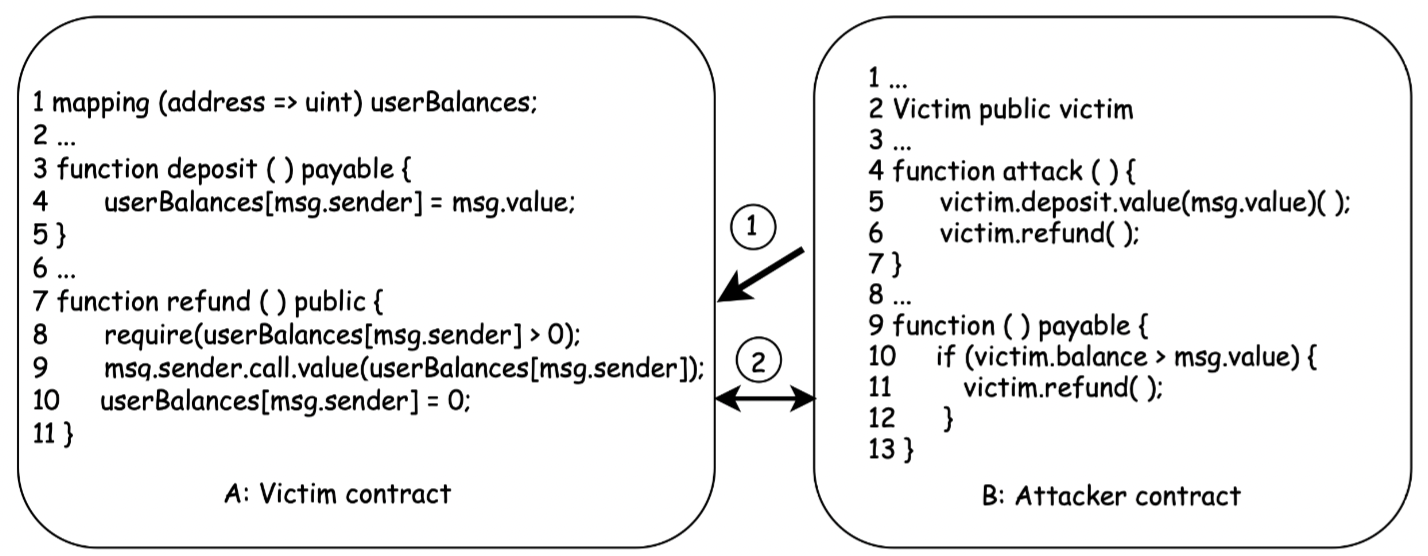
\includegraphics[width=0.8\textwidth]{image/pic1.png}
    \caption{重入漏洞漏洞的利用}
    \label{pic1}
\end{figure}

图\ref{pic1}显示了重入漏洞的利用方法。首先,调用攻击者智能合约中的 \textit{attack()} 函数向受害者合约存一些代币来调用受害者的脆弱 \textit{refund()})函数。然后,\textit{refund()})方法向攻击者合约(a中的第9行)发送申请的项目,也触发攻击合约中未命名的 \textit{fallback} 函数(B中的第9行)。 接下来,\textit{fallback}函数再次调用受害者合约中的\textit{refund()})函数(B中的第11行)。 由于受害者契约更新了\textit{userBalances}变量(A)之后的\textit{userbalances}变量(第10行)后,当攻击者重新进入\textit{refund()})函数时,\textit{userBalances}保持不变,因此仍然可以通过余额检查(a中的第8行)。因此,攻击者能够从受害者合约中反复转账,以此来盈利。

\subsection{缺少输入验证}

一个函数的参数在使用前应该被验证。如果开发者忘记给参数分配正确的值,EVM将使用基于参数类型的默认值来执行函数。这种机制使智能合约容易受到对函数参数的攻击。

\subsection{锁定代币}


2017年,一个脆弱的合约导致了百万美元的冻结。原因是这个合约依赖另一个库合约来提取其资金(使用delegatecall)。不幸的是,一个用户意外地从区块链上删除了该库合约(使用\textit{kill}指令),因此钱包合约中的资金无法再被提取。

\subsection{未处理的异常}

在 Solidity 中,有多种情况可能会引发异常。未处理的异常会影响智能合约的安全性。2016年2月,一个易受攻击的合约因为调用指令中存在未处理的异常,迫使所有者要求用户不要向所有者发送以太坊代币。

\subsection{算术漏洞}

以太坊虚拟机(EVM)为整数指定固定大小的数据类型。这意味着一个整型变量只能有一定范围的数字表示。例如,一个 \textit{uint8} ,只能存储在范围 [0,255] 的数字。试图存储 256 到一个 \textit{uint8} 将变成 0。不加注意的话,只要没有检查用户输入又执行计算,导致数字超出存储它们的数据类型允许的范围,Solidity 中的变量就可以被用来组织攻击。

整数溢出的类型包括乘法溢出,加法溢出,减法溢出三种。

\subsection{假EOS}

任何人都可以创建和发行名为EOS的令牌,因为在EOSIO中,令牌的名称和符号并不要求是唯一的。

由于\textit{eosio.token}的源代码是完全公开的,任何人都可以复制它的源代码并发行一个具有相同名称、符号和代码的令牌。然而,假的EOS和官方的EOS有不同的发行者。因此,如果攻击者通过复制合约的转移功能将假的EOS转移到赌博的DApp,DApp方收到的通知代码将不是\textit{eosio.token}。此外,如果DApp恰好没有检查代码的值,那么调度器中的验证将被绕过。

为了缓解上述问题,一些开发者缩小了接受代码的范围。\textit{self} 或 \textit{eosio.token} 都可以被当作代码的有效输入值。然而,如果攻击者直接调用转移函数,这样的缓解措施也可以被绕过。
由于条件 \textit{code == self} 总是被满足,即使没有来自eosio.token的通知,转移函数也会被调用,这表明有转移请求。

这两种情况都属于假EOS令牌漏洞\cite{7}。

\subsection{假收据}

如果DApp开发者对代码进行了全面的检查,那么通知就会被调度器转发。但是,如果开发者在这一步没有进行核查,DApp就会被攻击。
需要强调的是,通知可以被转发,而代码不会改变。因此,DApp可能被同时扮演发起人和共犯双重角色(账户)的攻击者所欺骗。具体来说,发起人通过\textit{eosio.token}向共犯(用\textit{to}表示,转移函数的参数)调用常规转移。当帮凶收到\textit{eosio.token}的通知时,它将立即把通知转发给DApp,而不作任何修改。通过这种方式,代码没有改变,这仍然是官方的发行者:\textit{eosio.token}。因此,调度器将不知道任何异常情况。然而,如果在转移中不检查参数\textit{to},DApp将被愚弄,因为代币转移在攻击者控制的两个账户之间完成。
这可能会导致DApp开发者的直接经济损失。

\subsection{回滚漏洞}

在\textit{reveal}函数中,DApp处理与玩家的转移一起收到的赌注。在转移函数中,开发者通常使用各种链上状态值作为种子(例如,\textit{current\_time},表示执行动作时的时间戳)来生成一个伪随机数3,最后通过\textit{modulo operation}将生成的数字与玩家的输入进行比较来获得结果,这是由Wasm字节码中的\textit{rem}操作符实现的。注意,一般来说,回滚的情况只能在赌博的DApps中找到。我们假设它总是在那里,并且可以从调度器中到达。
即使开发者对输入的每个参数都做了彻底的检查,并在任何敏感动作之前检查调用者的权限,一个符合图3模型的游戏仍然可能被攻击。具体来说,所有的动作都是内联调用的,也就是说,在一个交易中定位。因此,当玩家在第8步后收到通知时,他可以立即调用另一个内联动作到\textit{eosio.token}来检查他的余额。如果他的余额减少,那么就意味着他没有赢得这一轮。他可以使用一个断言语句来迫使当前的动作失败。一个动作的失败可能会导致整个交易的逆转。通过这种方式,玩家可以继续尝试,直到他中了大奖。我们把这种恶意的回滚称为回滚漏洞。

\section{漏洞检测}

以上我们列出来在Ethereum和EOSIO平台上的常见漏洞,下面我们将介绍如何检测以上漏洞。

\subsection{通过比较历史版本检测漏洞}

对于以太坊来说,在区块链系统上摧毁智能合约的唯一方法是在攻击者发现漏洞时使用 \textit{Selfdestruct} 函数。
与以太坊不同,部署在基于EOSIO的区块链上的应用程序是可以更新的。
这意味着只要提供足够的权限,你就可以部署代码修复的补丁,增加功能,并改变应用程序的逻辑。
作为一个开发者,你可以迭代你的应用程序,而不会有被永久锁定在一个软件错误中的风险。
我们可以很容易地收集同一智能合约的几个版本。
一般来说,开发者更新的代码可能是漏洞、新功能,甚至是人为植入的欺诈代码。

\subsection{符号执行}

EOSafe将符号执行引擎设计为泛型框架,以模拟基于堆栈的EOS VM上的智能合同的执行。它接受CFG和拆卸的WASM指令作为输入,并在基本块中进行符号执行,以便以获取所有可行的路径。在此过程中,相应地生成路径约束。具体地,模块维护两个关键组件:路径树和状态。路径树由路径组成,可以进行当前智能合同的可控制流程。当遇到某些条件指令(如\textit{br\_table})时,路径将分为两条路径。沿着每条路径,我们不仅记录相应的约束(即控制流的输入值的条件导致该结果),还有调用的导入功能的所有签名,这有助于分析漏洞检测。至于该状态,我们维护了一些必要的状态相关信息,包括本地/全局变量,线性存储器,堆栈和随后的指令,以及其对应的程序计数器。

\subsection{模糊测试}

\begin{figure}[htbp]
    \centering
    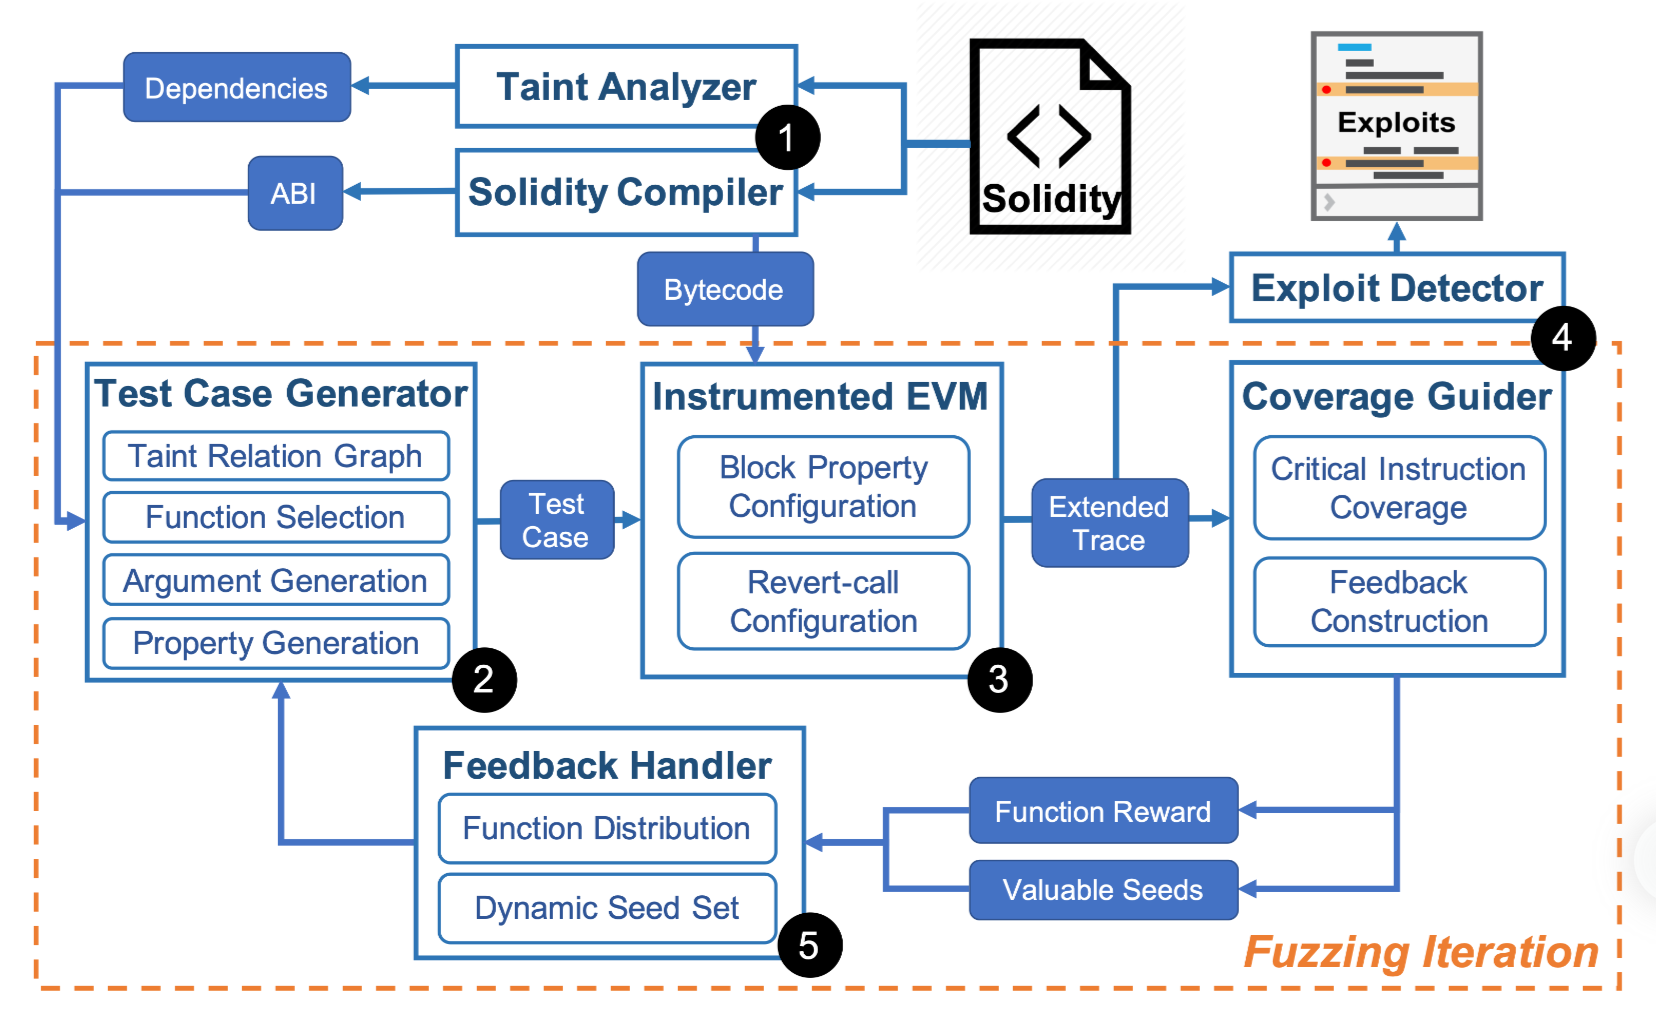
\includegraphics[width=0.8\textwidth]{image/pic2.png}
    \caption{ETHPLOIT的工作流}
    \label{pic2}
\end{figure}

一些研究者设计了一个用于自动分析智能合同的模糊工具ETHPLOIT\cite{8}。其中包括五个步骤:

\begin{enumerate}
    \item 静态分析。鉴于智能合同的稳定性代码,Ethploit编译了提取应用程序二进制接口(ABI)和字节码的代码。它还适用Taint分析来提取变量之间的依赖性。
    \item 测试案例。 Ethploit最初生成测试用例。 Ethploit而不是提供任何预定义的代码模式,而是进行模糊以优化测试用例。基于前一轮模糊测试产生的静态分析结果和反馈结果,进一步更新测试案例。
    \item 测试案例执行。 Ethploit Instruments是模拟区块链效应的EVM。它还在仪表EVM和输出执行跟踪上应用每个测试用例。由于指令,迹线涵盖了更多的执行概率。
    \item 追踪分析。 Ethploit分析每个执行跟踪。如果Exproit检测器标识漏洞利用,则Ethploit将当前的测试用例报告为有效的漏洞利用。同时,指令的覆盖范围作为反馈构建优化测试用例。ETHPLOIT将反馈区分为两类:修改功能分布和用于更新动态种子集的有价值种子的功能奖励。
    \item 反馈处理。 Ethploit将功能奖励视为测试案例发生器的功能分布,以选择更有可能通过过去模糊迭代的经验利用漏洞的功能。
\end{enumerate}

反馈处理程序还将有价值的种子添加到种子集中,该种子集可用于生成能够解决一些严格约束的参数。

\subsection{根据现有工具进行投票制筛选}

在漏洞修复框架EVMPATCH\cite{9}中,在能够应用修补程序之前,EVMPATCH框架需要识别和检测漏洞。为此,EVMPATCH框架利用现有的漏洞检测工具,例如[\cite{10},\cite{11},\cite{12},\cite{13},\cite{14},\cite{15},\cite{16}]。 对于任何现有工具未检测到的漏洞,要求开发人员或安全顾问创建漏洞报告。 在EVMPATCH的系统中,漏洞检测组件负责标识漏洞所在的指令的确切地址,以及漏洞的类型。然后将该信息传递给字节码重写器,相应地修补合同。

\section{漏洞自动修复}

目前调研有大概这样的漏洞自动修复方法。

\begin{itemize}
    \item 使用基于模板的修复模式生成补丁\cite{17},并利用静态程序分析。
    \item 二进制重写\cite{9}。二进制重写也被应用于改造安全加固技术,如控制流的完整性,以编译的二进制文件,但也可以动态地将安全补丁应用于运行的程序。对于传统架构上的二进制重写,已经开发了两种类型的方法:静态和动态重写。
\end{itemize}

不过漏洞自动修复还不算成熟,泛用性不够。目前市面上的区块链公司仍采用专业人员代码审计。

\section{评估}

大体上,相关工作的评估方面有以下几种:

\begin{itemize}
    \item 假阳性
    \item 是否会引入新的漏洞
    \item 运行时性能
    \item 额外Gas开销
\end{itemize}

\section{总结}

区块链上的智能合约仍存在着大量漏洞,漏洞的检测和修复手段也在发展中,相关漏洞带来的经济损失惨重,未来这个方面仍是重要的科研方向。


%%%%%%%%%%%%%%%%%%%%%%%%%%%%%%%%%%%%%%%%%%%%%%%%%%%%%%%
%%% 参考文献, {}为引用的标签, 数字/字母均可
%%% 文中上标引用: \upcite{1,2}
%%% 文中正常引用: \cite{1,2}
%%%%%%%%%%%%%%%%%%%%%%%%%%%%%%%%%%%%%%%%%%%%%%%%%%%%%%%
\newpage

\begin{thebibliography}{99}

    \bibitem{1} Ethereum[EB/OL].https://ethereum.org/en/.

    \bibitem{2} EOSIO Developer Portal[EB/OL].https://developers.eos.io/.

    \bibitem{3} EOSRoyale Smart Contract. https://www.eosroyale.com, Last access, 2020.

    \bibitem{4} Analysis of the DAO exploit. http://hackingdistributed.com/2016/06/18/analysis-of-the-daoexploit/. Last access, 2020.

    \bibitem{5} CRAIG RUSSO, "EOSIO surpasses Ethereum in transaction volume," Sep. 2018. [Online]. Available: https://sludgefeed.com/eos-surpasses-ethereum-in -daily-dapp-users-and-transaction-volume/

    \bibitem{6} Alfredo de Candia, "Increase of EOSIO transaction volumes," Sep. 2019. [Online]. Available: https://en.crypt onomist.ch/2019/09/03/eos-porn-transaction-volumes

    \bibitem{7} He, N. ,  Zhang, R. ,  Wu, L. ,  Wang, H. ,  Luo, X. , \&  Guo, Y. , et al. (2020). Security analysis of eosio smart contracts.

    \bibitem{8} Zhang, Q. ,  Wang, Y. ,  Li, J. , \&  Ma, S. . (2020). EthPloit: From Fuzzing to Efficient Exploit Generation against Smart Contracts. 2020 IEEE 27th International Conference on Software Analysis, Evolution and Reengineering (SANER). IEEE.

    \bibitem{9} Rodler, M. ,  Li, W. ,  Karame, G. O. , \&  Davi, L. . (2020). Evmpatch: timely and automated patching of ethereum smart contracts.

    \bibitem{10} Christof Ferreira-Torres, Julian Schütte, and Radu State. "Osiris: Hunting for Integer Bugs in Ethereum Smart Contracts". In: Proceedings of the 34th Annual Computer Security Applications Conference (ACSAC).2018. DOI: 10.1145/3274694.3274737.

    \bibitem{11} Shelly Grossman, Ittai Abraham, Guy Golan-Gueta, Yan Michalevsky, Noam Rinetzky, Mooly Sagiv, and Yoni Zohar. "Online detection of effectively callback free objects with applications to smart contracts".In: Proceedings of the ACM on Programming Languages POPL (2018).DOI: 10.1145/3158136.

    \bibitem{12} Johannes KruppandChristian Rossow. "teEther: Gnawing atEthereum to Automatically Exploit Smart Contracts". In: 27th USENIX Security Symposium. USENIX Association, 2018. URL: https://www.usenix.org/conference/usenixsecurity18/presentation/ krupp.

    \bibitem{13} Loi Luu, Duc-Hiep Chu, Hrishi Olickel, Prateek Saxena, and Aquinas Hobor. "Making smart contracts smarter". In: Proceedings of the ACM SIGSAC Conference on Computer and Communications Security (CCS). ACM. 2016.

    \bibitem{14} Ivica Nikolic, Aashish Kolluri, Ilya Sergey, Prateek Saxena, and Aquinas Hobor. "Finding The Greedy, Prodigal, and Suicidal Contracts at Scale". In: 34th Annual Computer Security Applications Conference (ACSAC). 2018. DOI: 10.1145/3274694.3274743.

    \bibitem{15} Michael Rodler, Wenting Li, Ghassan O. Karame, and Lucas Davi."Sereum: Protecting Existing Smart Contracts Against Re-Entrancy Attacks". In: Proceedings of the Network and Distributed System Security Symposium (NDSS). 2019. DOI: 10.14722/ndss.2019.23413.

    \bibitem{16} Petar Tsankov, Andrei Dan, Dana Drachsler-Cohen, Arthur Gervais, Florian Buenzli, and Martin Vechev. "Securify: Practical security analysis of smart contracts". In: Proceedings of the 2018 ACM SIGSAC Conference on Computer and Communications Security. 2018.

    \bibitem{17} Nguyen, T. D. ,  Pham, L. H. , \&  Sun, J. . (2021). Sguard: towards fixing vulnerable smart contracts automatically.

\end{thebibliography}

%%%%%%%%%%%%%%%%%%%%%%%%%%%%%%%%%%%%%%%%%%%%%%%%%%%%%%%
%%% 附录章节, 自动从A编号, 以\section开始一节
%%% 非必选
%%%%%%%%%%%%%%%%%%%%%%%%%%%%%%%%%%%%%%%%%%%%%%%%%%%%%%%
%\begin{appendix}
%\section{附录}
%附录从这里开始.
%\begin{figure}[H]
%\centering
%%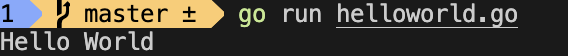
\includegraphics{fig1.eps}
%\cnenfigcaption{附录里的图}{Caption}
%\label{fig1}
%\end{figure}
%\end{appendix}


%%%%%%%%%%%%%%%%%%%%%%%%%%%%%%%%%%%%%%%%%%%%%%%%%%%%%%%
%%% 自动生成英文标题部分
%%%%%%%%%%%%%%%%%%%%%%%%%%%%%%%%%%%%%%%%%%%%%%%%%%%%%%%
% \makeentitle


%%%%%%%%%%%%%%%%%%%%%%%%%%%%%%%%%%%%%%%%%%%%%%%%%%%%%%%
%%% 补充材料, 以附件形式作网络在线, 不出现在印刷版中
%%% 不做加工和排版, 仅用于获得图片和表格编号
%%% 自动从I编号, 以\section开始一节
%%% 可以没有\section
%%%%%%%%%%%%%%%%%%%%%%%%%%%%%%%%%%%%%%%%%%%%%%%%%%%%%%%
%\begin{supplement}
%\section{supplement1}
%自动从I编号, 以section开始一节.
%\begin{figure}[H]
%\centering
%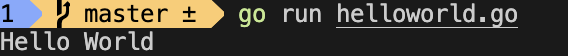
\includegraphics{fig1.eps}
%\cnenfigcaption{补充材料里的图}{Caption}
%\label{fig1}
%\end{figure}
%\end{supplement}

\end{document}
